\documentclass[UTF8,a4paper,11pt]{ctexart}

\usepackage[a4paper,margin=2.4cm]{geometry}
\usepackage{graphicx}
\usepackage{booktabs}
\usepackage{tabularx}
\usepackage{longtable}
\usepackage{array}
\usepackage{amsmath}
\usepackage{xcolor}
\usepackage{enumitem}
\usepackage{hyperref}
\usepackage{caption}
\usepackage{subcaption}
\usepackage{float}

\hypersetup{
  colorlinks=true,
  linkcolor=blue!55!black,
  urlcolor=blue!55!black,
  citecolor=blue!55!black
}
\setlist[itemize]{leftmargin=1.8em}
\setlist[enumerate]{leftmargin=1.8em}
\graphicspath{
  {../results/parameter_variants/common/}
  {../results/parameter_variants/paper_text/}
  {../results/parameter_variants/original_notebook/}
  {../results/}
}

\title{《Queues under Stochastic Priority Switching》复现报告}
\author{Stochastic Operations Research 复现项目}
\date{2026年6月}

\newcommand{\code}[1]{\texttt{#1}}
\newcommand{\pass}{\textcolor{green!45!black}{成功}}
\newcommand{\partialpass}{\textcolor{orange!70!black}{部分成功}}
\newcommand{\fail}{\textcolor{red!65!black}{未确认}}

\begin{document}
\maketitle

\begin{abstract}
本报告基于当前仓库中的完整实验输出，对 Palmer 等人的随机优先级切换队列模型复现工作进行复核。总体结论是：复现工程链路已经基本完成，主要脚本均能产生可审计的 CSV 指标表和 PNG 图；有限截断 Markov 链近似、原始 notebook 参数下的稳定性实验、部分 $H$ 矩阵热图和 sojourn-time 二阶矩分析具有较好的复现效果。但是，当前结果不能简单写成“完全复现成功”：Figure 5 中论文候选点 $(\theta_{12},\theta_{21})=(3,1)$ 没有在当前仿真中成为最优点；论文文本参数下的稳定性 ADF 检验未能判定 stable-like 轨迹平稳；Scenario A 的 $Q(16)$ 边界量明显超过论文阈值。新增的综合校准指标适合作为扩展实验中的探索性筛选工具，但不应替代论文原始指标。
\end{abstract}

\tableofcontents
\newpage

\section{复现目标与总体判断}

本复现工作的目标不是只生成相似图片，而是确认以下三个层面是否成立：

\begin{enumerate}
  \item \textbf{模型与代码链路是否可运行：} 能否从原始代码、原始数据和论文参数出发，重新生成主要实验结果。
  \item \textbf{数值结论是否复现：} 论文中关于 overtaking 分布、稳定性、有限边界 Markov 近似、切换率矩阵 $H$ 影响等结论是否在当前实现中得到支持。
  \item \textbf{扩展是否合理：} 新增的 finer-grid calibration、Markov-vs-simulation 检查、sojourn-time variance 可视化是否与原模型逻辑一致，是否会混淆复现口径。
\end{enumerate}

当前结论可以概括为“\textbf{工程复现完成，数值复现混合成功}”。其中，Bounded Markov approximation 是最稳定、证据最强的部分；原始 notebook 参数下的稳定性实验也能复现 stable/unstable 的 ADF 区分。但 Figure 5、论文文本参数下的稳定性、Scenario A 的边界量存在明显 caveat。因此，在最终汇报中建议使用“部分复现成功，并发现若干参数与随机性敏感点”的表述，而不是“完全复现论文全部数值结论”。

\section{代码架构与结果目录}

\subsection{复现代码结构}

复现层位于 \path{reproduction/}，没有直接改写原始模型库，而是以包装脚本的方式调用 \path{archive/original/src} 中的原始模型函数。主要模块如下：

\begin{longtable}{@{}p{0.34\textwidth}p{0.57\textwidth}@{}}
\toprule
模块 & 作用 \\
\midrule
\path{reproduction/utils.py} & 统一处理路径、原始手术等待数据、class-switching rate 的零值语义、Ciw 仿真、overtaking 指标。\\
\path{reproduction/reproduce_figure5.py} & 复现论文 Figure 5 风格的 overtaking 分布比较，输出 Wasserstein distance 和等待时间 MAPE。\\
\path{reproduction/reproduce_stability.py} & 对 stable-like 与 unstable-like 轨迹做 ADF 检验，用于复核稳定性现象。\\
\path{reproduction/reproduce_bounded_markov.py} & 计算有限边界 Markov 链下的 $L$、$W$、$Q(b)$、$P(b)$ 随 bound 的变化。\\
\path{reproduction/reproduce_effect_of_H.py} & 在 $h_{12}\times h_{21}$ 网格上计算 $L_k$、$W_k$、sojourn-time variance $U$ 与边界量。\\
\path{reproduction/reproduce_mc_vs_sim.py} & 比较 bounded Markov chain 与离散事件仿真的状态分布和 sojourn-time 均值。\\
\path{reproduction/reproduce_sojourn_variance.py} & 复核吸收 Markov 链二阶矩公式，并生成 variance convergence 与 heatmap。\\
\path{reproduction/extension_calibrate_H.py} & 扩展实验：使用更细的 $H$ 网格和综合校准损失探索拟合面。\\
\path{reproduction/run_parameter_variants.py} & 针对论文文本和原始 notebook 参数不一致处分别运行，避免混用口径。\\
\bottomrule
\end{longtable}

\subsection{结果目录}

本轮完整实验结果主要位于：

\begin{itemize}
  \item \path{../results/parameter_variants/common/}：无明显论文文本/原 notebook 参数冲突的共同实验，包括 Figure 5 和 effect-of-$H$。
  \item \path{../results/parameter_variants/paper_text/}：采用论文文本参数的 bounded Markov、stability、MC-vs-sim、variance 实验。
  \item \path{../results/parameter_variants/original_notebook/}：采用原始 notebook 参数的对应实验。
  \item \path{../results/extension_calibration/}：扩展校准实验。
\end{itemize}

早期输出已按实验类型归类至 \path{../results/} 的子目录（\path{figure5/}、\path{effect_of_H/}、\path{bounded_markov/}、\path{mc_vs_sim/}、\path{sojourn_variance/}）中。这些文件可能来自修正之前的版本，最终分析应优先采用 \path{../results/parameter_variants/} 下的新输出。

\section{参数口径：论文文本 vs 原始 notebook}

本次复现中一个关键处理是将论文文本参数和原始 notebook 参数分开运行。这样做是合理且必要的，因为部分实验的参数来源存在不一致：

\begin{table}[H]
\centering
\caption{需要区分的参数口径}
\begin{tabularx}{\textwidth}{@{}p{0.24\textwidth}p{0.23\textwidth}p{0.23\textwidth}X@{}}
\toprule
实验 & 论文文本口径 & 原始 notebook 口径 & 影响 \\
\midrule
稳定性实验 & $\theta_{12}=3,\theta_{21}=1$ & $\theta_{12}=2,\theta_{21}=1$ & ADF 检验结论不同；notebook 口径能复现 stable/unstable 区分。\\
Bounded Markov、MC-vs-sim、variance & $\mu_2=2.5$ & $\mu_2=1.6666666667$ & 两者均收敛，但 $L$、$W$ 的数值水平不同。\\
Figure 5 与 effect-of-$H$ & 共同运行 & 共同运行 & 当前脚本中没有作为参数变体拆分。\\
\bottomrule
\end{tabularx}
\end{table}

因此，最终报告中建议同时呈现两版：论文文本版用于对照论文叙述，原始 notebook 版用于判断作者代码路径能否复现。若只采用其中一版，容易把参数差异误解为代码错误或实验失败。

\section{逐项复现结果}

\subsection{Figure 5：overtaking 分布拟合}

Figure 5 复现实验使用原始仓库中的手术等待列表数据作为 observed target，通过 Ciw 仿真生成 overtaking distribution，并在粗网格
\[
  \theta_{12}\in\{1,2,3\},\qquad \theta_{21}\in\{0,1,2\}
\]
上比较 Wasserstein distance 与 waiting-time MAPE。注意：这两个指标是论文复现口径，应分别报告；不应在 Figure 5 复现实验中用新增综合指标替代。

\begin{figure}[H]
\centering
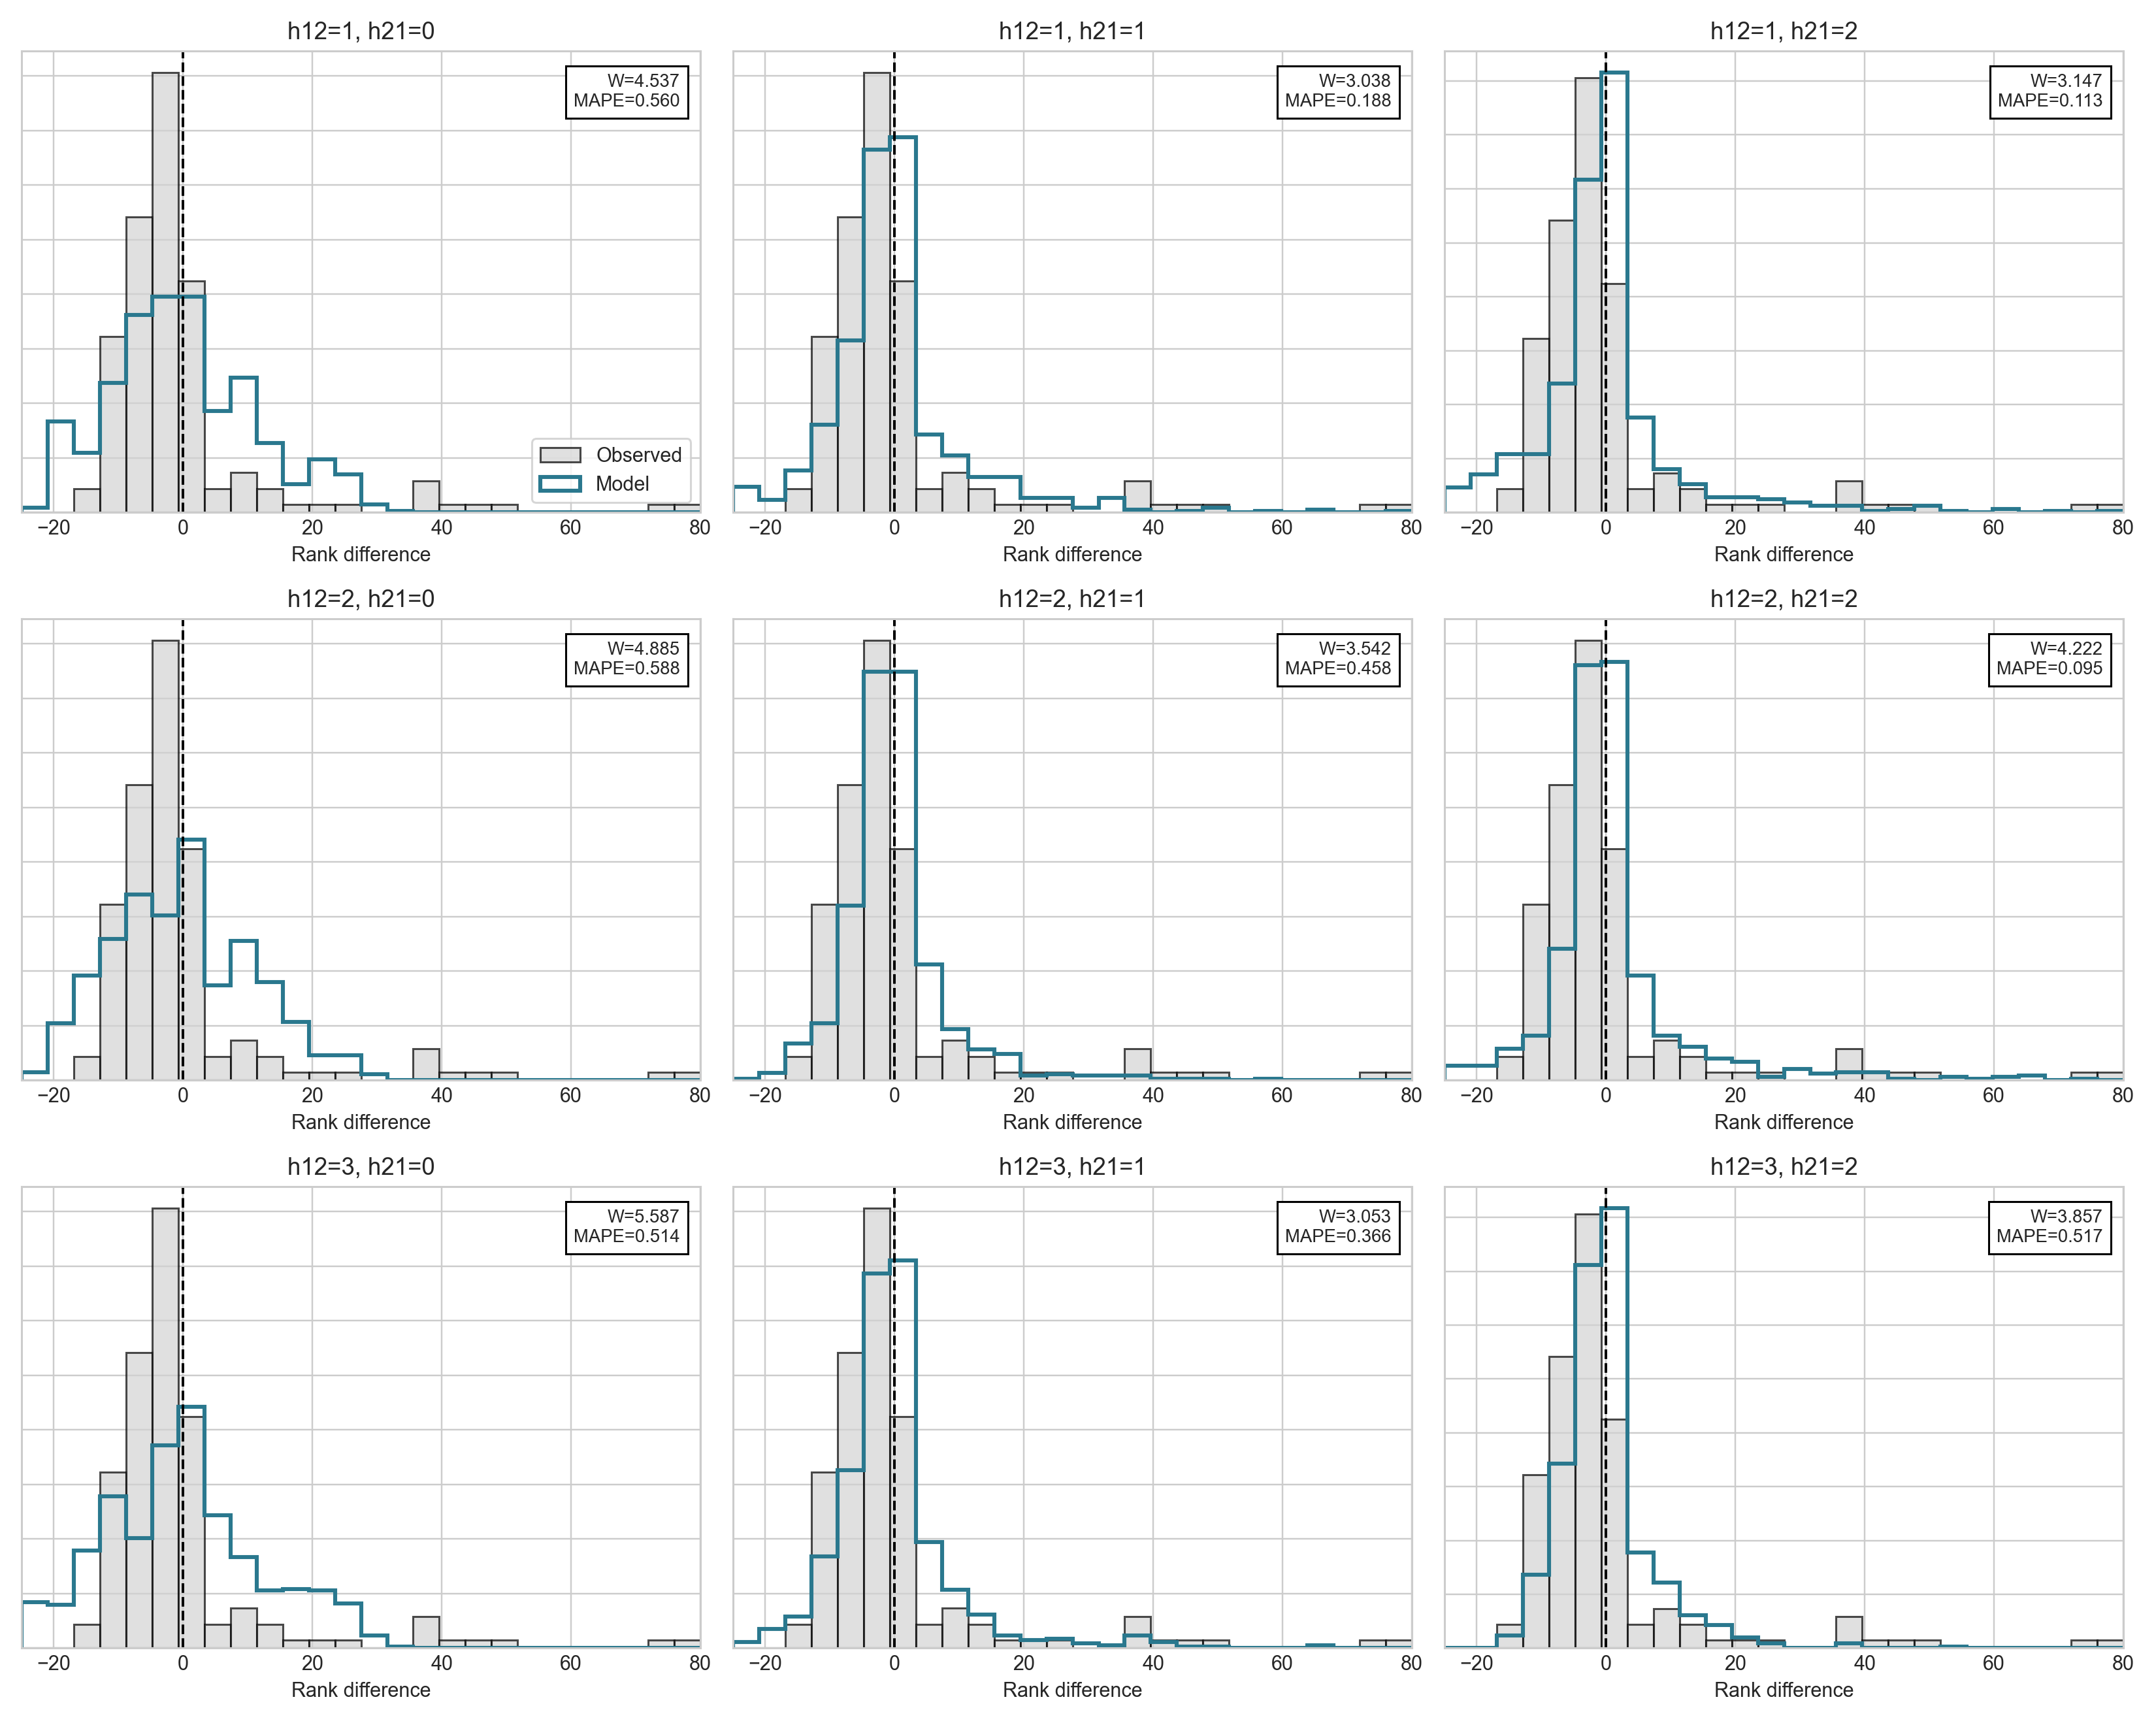
\includegraphics[width=0.88\textwidth]{../results/parameter_variants/common/figure5_replication.png}
\caption{Figure 5 风格的 overtaking 分布复现图。}
\end{figure}

当前 CSV 结果显示：

\begin{table}[H]
\centering
\caption{Figure 5 当前主要结果}
\begin{tabular}{@{}lccc@{}}
\toprule
判据 & 最优或关注点 & Wasserstein & MAPE \\
\midrule
最小 Wasserstein & $(1,1)$ & 3.0381 & 0.1879 \\
论文候选点 & $(3,1)$ & 3.0528 & 0.3663 \\
最小 MAPE & $(2,2)$ & 4.2217 & 0.0946 \\
次低 MAPE 附近 & $(1,2)$ & 3.1471 & 0.1128 \\
\bottomrule
\end{tabular}
\end{table}

\textbf{判断：\partialpass。} 当前复现成功运行了论文式比较流程，也生成了合理的分布图。但是论文候选点 $(3,1)$ 在当前 run 中没有成为最小 Wasserstein 点，也不是最小 MAPE 点。它的 Wasserstein 与最优点非常接近，说明分布形状上并非完全不合理；但 MAPE 明显更差，因此不能把当前结果写成 Figure 5 关键结论完全复现。

可能原因包括：仿真随机性、trial 数较少、Ciw 版本差异、原始数据处理细节、论文图中是否采用更多重复仿真或平滑处理等。若要加强该结论，需要增加 trials、固定更多随机种子并报告置信区间或 seed sensitivity。

\subsection{稳定性实验与 ADF 检验}

稳定性实验对 stable-like 与 unstable-like 两类队列长度轨迹做 ADF 检验。当前结果如下：

\begin{table}[H]
\centering
\caption{稳定性实验 ADF 结果}
\begin{tabular}{@{}lcccc@{}}
\toprule
参数口径 & stable-like ADF $p$ & stable-like 末端队长 & unstable-like ADF $p$ & unstable-like 末端队长 \\
\midrule
论文文本 & 0.1562 & 10 & 0.8558 & 241 \\
原始 notebook & 0.00385 & 0 & 0.8639 & 144 \\
\bottomrule
\end{tabular}
\end{table}

\begin{figure}[H]
\centering
\begin{subfigure}{0.48\textwidth}
\centering
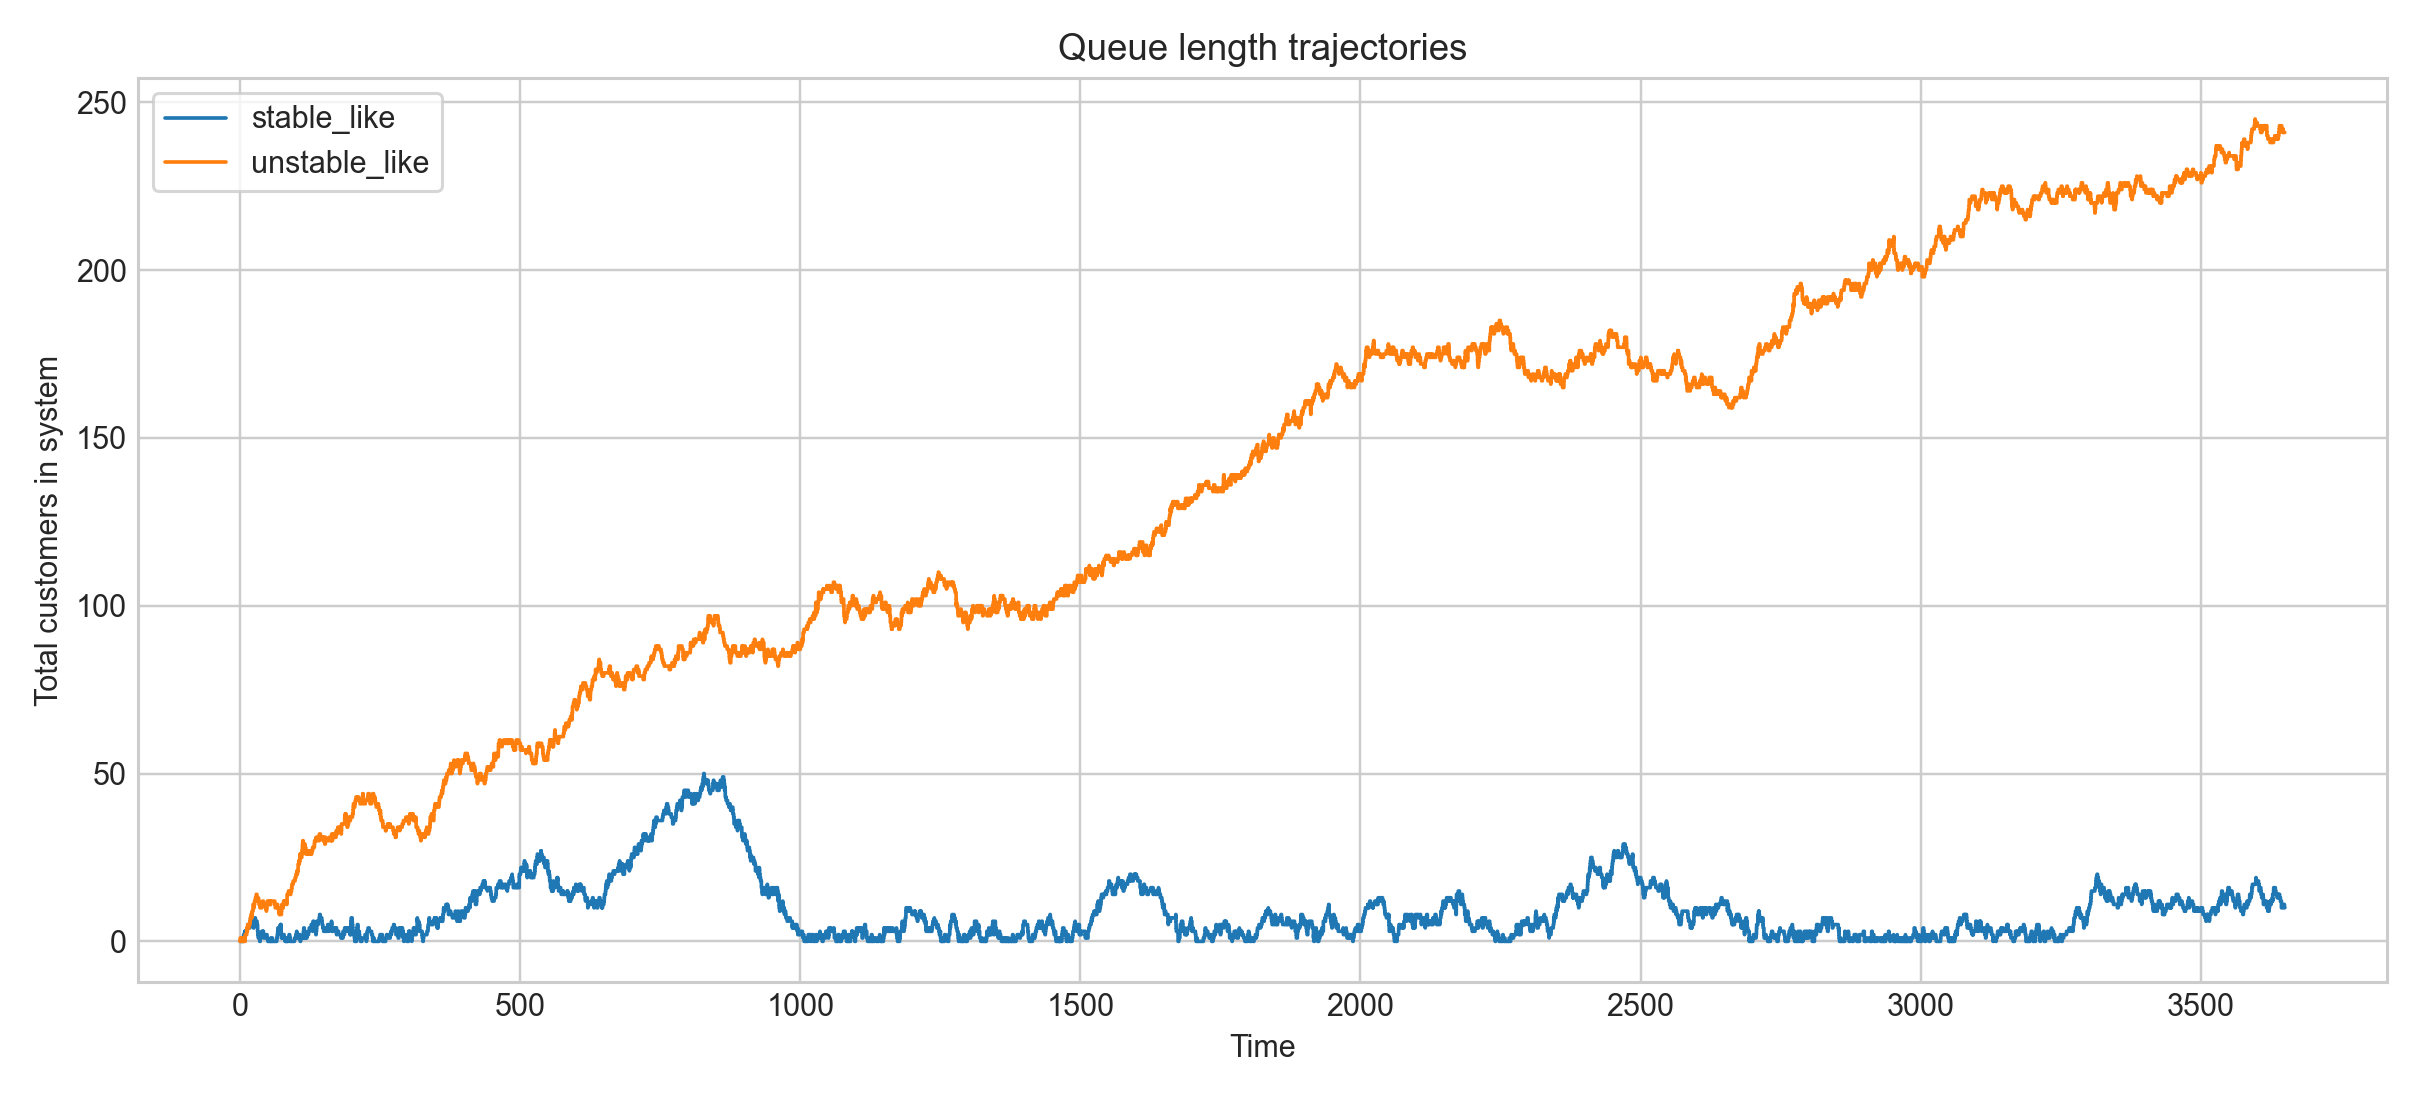
\includegraphics[width=\textwidth]{../results/parameter_variants/paper_text/stability_replication.png}
\caption{论文文本参数}
\end{subfigure}
\hfill
\begin{subfigure}{0.48\textwidth}
\centering
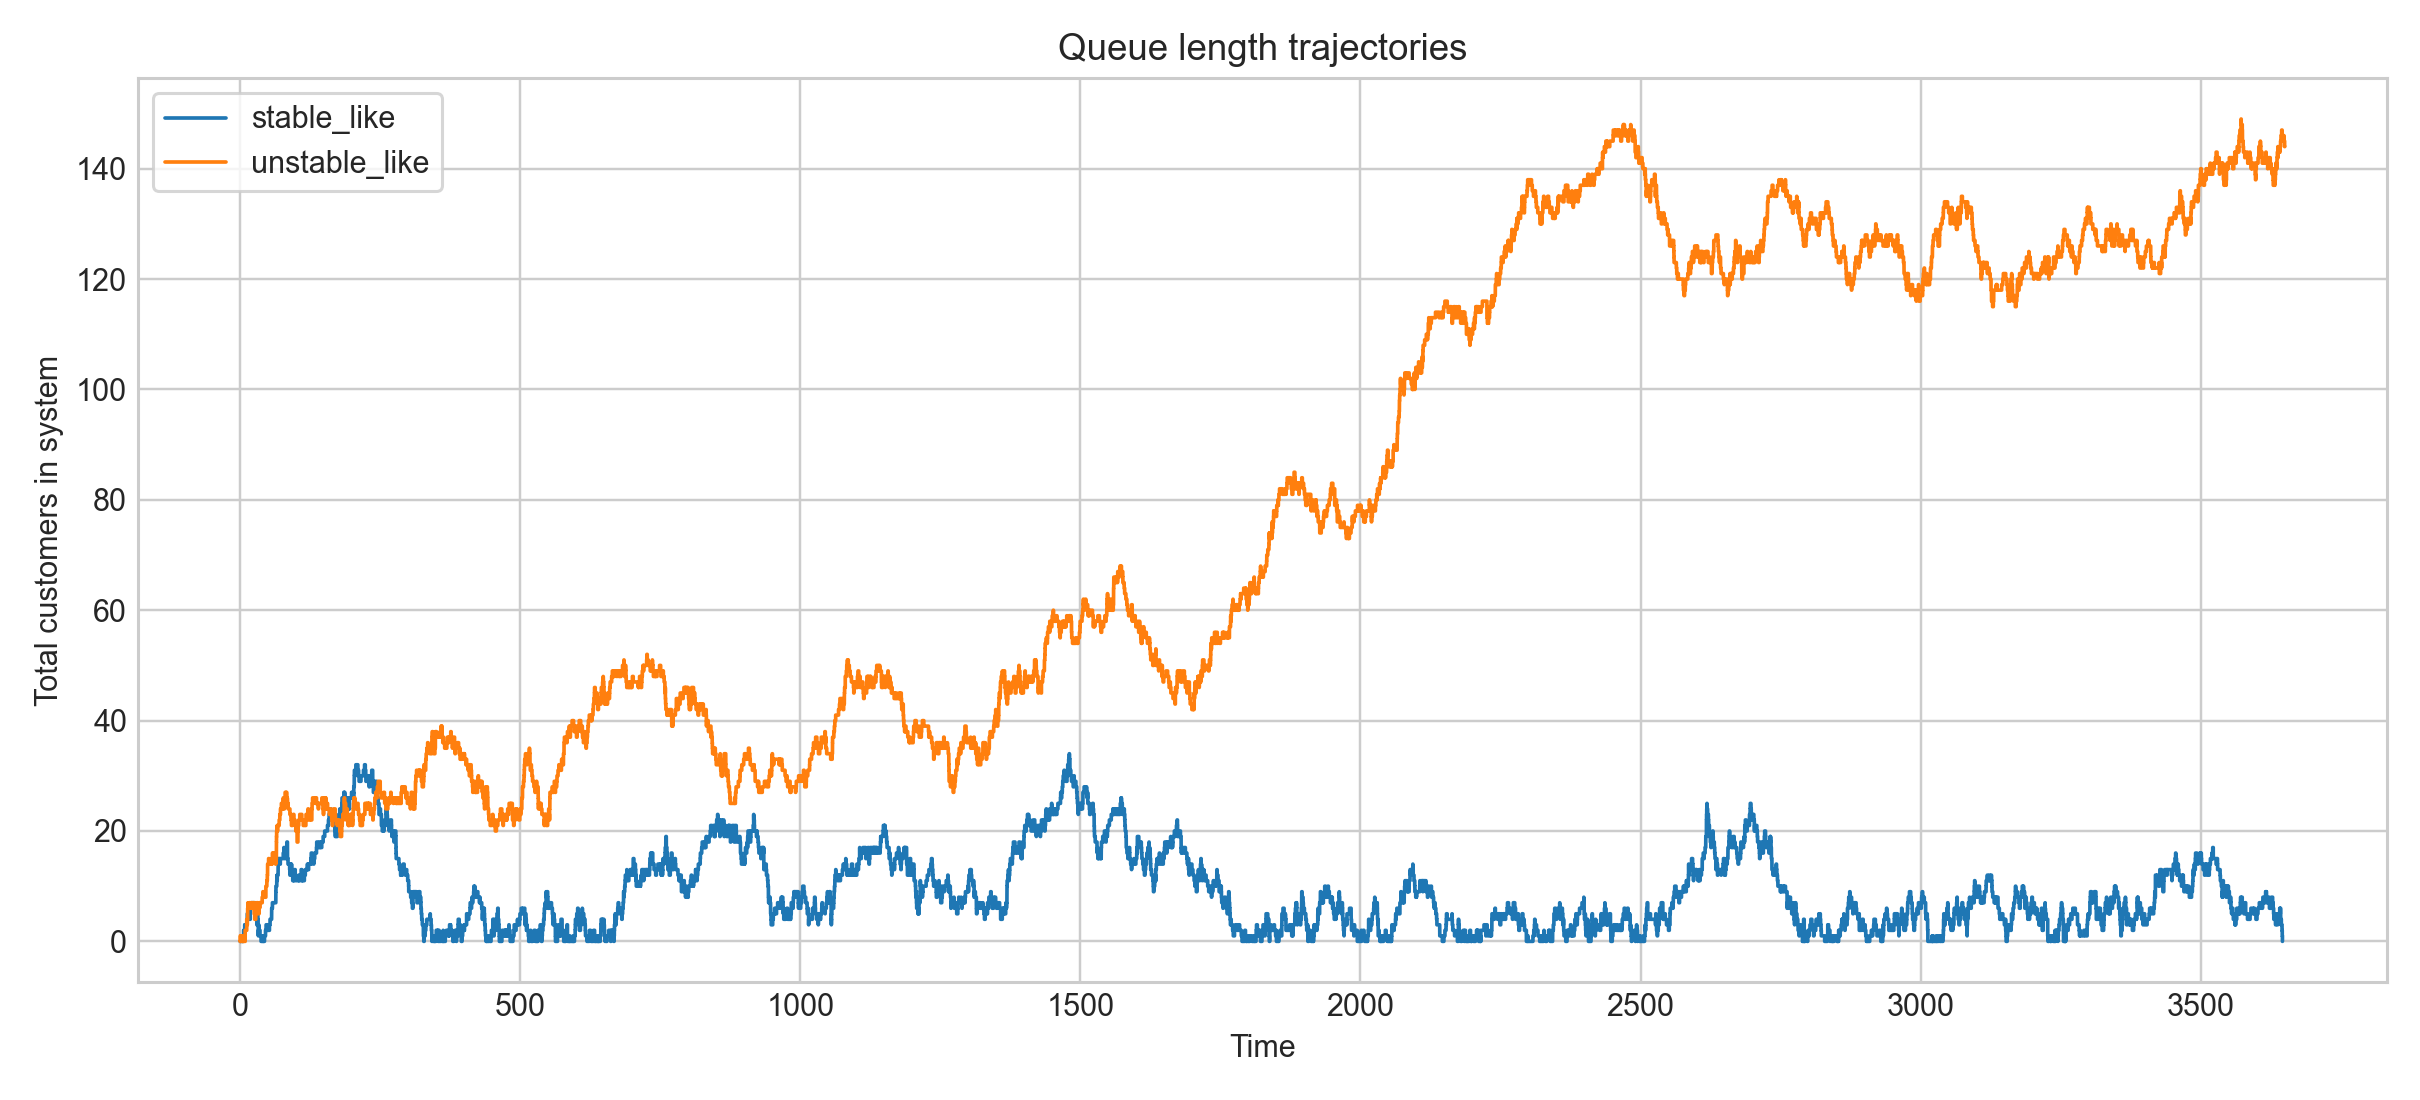
\includegraphics[width=\textwidth]{../results/parameter_variants/original_notebook/stability_replication.png}
\caption{原始 notebook 参数}
\end{subfigure}
\caption{稳定性复现的两种参数口径。}
\end{figure}

\textbf{判断：\partialpass。} 原始 notebook 参数下，stable-like 的 ADF $p=0.00385<0.05$，unstable-like 的 $p=0.8639$，符合“一个平稳、一个非平稳”的预期。论文文本参数下，unstable-like 仍然明显非平稳，但 stable-like 的 ADF $p=0.1562$，不能拒绝单位根；这意味着按严格 ADF 口径，论文文本版没有完全复现。

因此，汇报时建议写为：稳定性现象在原 notebook 口径下复现，在论文文本口径下视觉上不爆炸但统计检验不充分。

\subsection{有限边界 Markov 链近似}

Bounded Markov 实验计算不同截断 bound 下的平均系统人数 $L$、平均 sojourn time $W$，以及边界相关量 $Q(b)$、$P(b)$。当前两种参数口径在 $b=22$ 时结果为：

\begin{table}[H]
\centering
\caption{Bounded Markov 在 $b=22$ 的结果}
\begin{tabular}{@{}lccccc@{}}
\toprule
参数口径 & $\mu_2$ & $L$ & $W$ & $Q(b)$ & $P(b)$ \\
\midrule
论文文本 & 2.5 & 1.6197 & 1.6199 & $5.88\times10^{-5}$ & $2.39\times10^{-5}$ \\
原始 notebook & 1.6667 & 1.9158 & 1.9161 & $7.61\times10^{-5}$ & $3.10\times10^{-5}$ \\
\bottomrule
\end{tabular}
\end{table}

\begin{figure}[H]
\centering
\begin{subfigure}{0.48\textwidth}
\centering
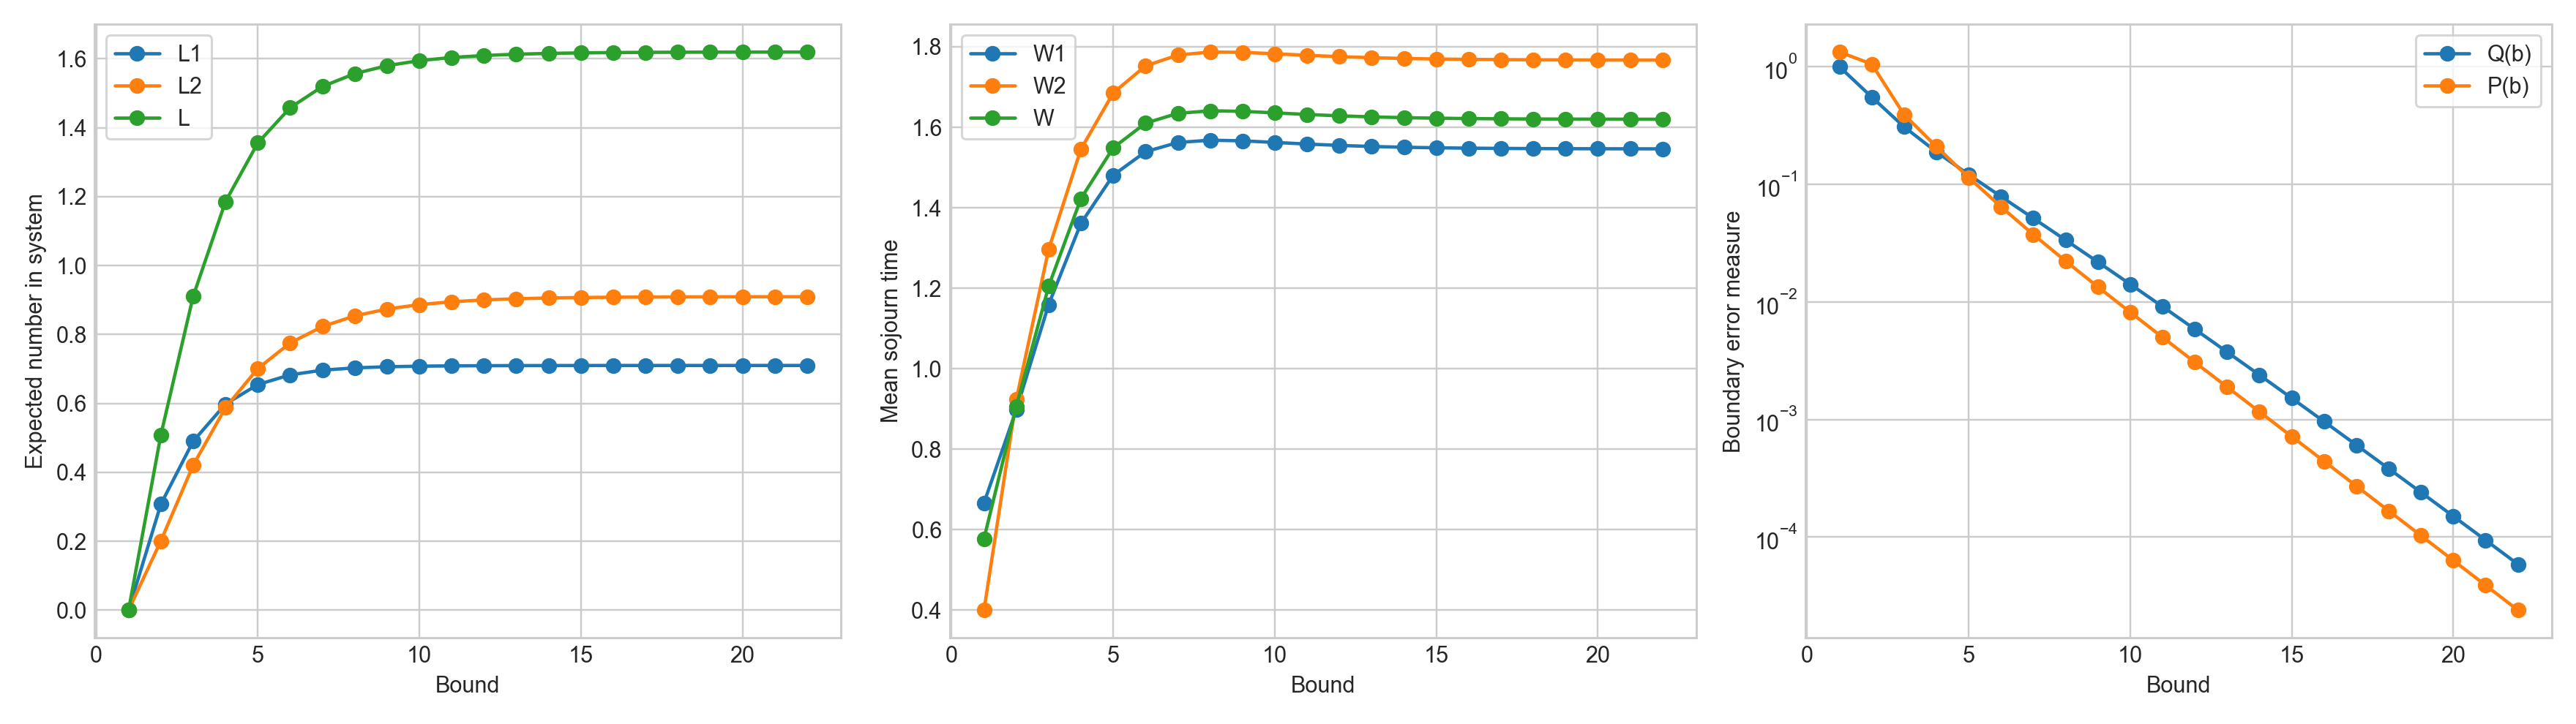
\includegraphics[width=\textwidth]{../results/parameter_variants/paper_text/bounded_markov_replication.png}
\caption{论文文本参数}
\end{subfigure}
\hfill
\begin{subfigure}{0.48\textwidth}
\centering
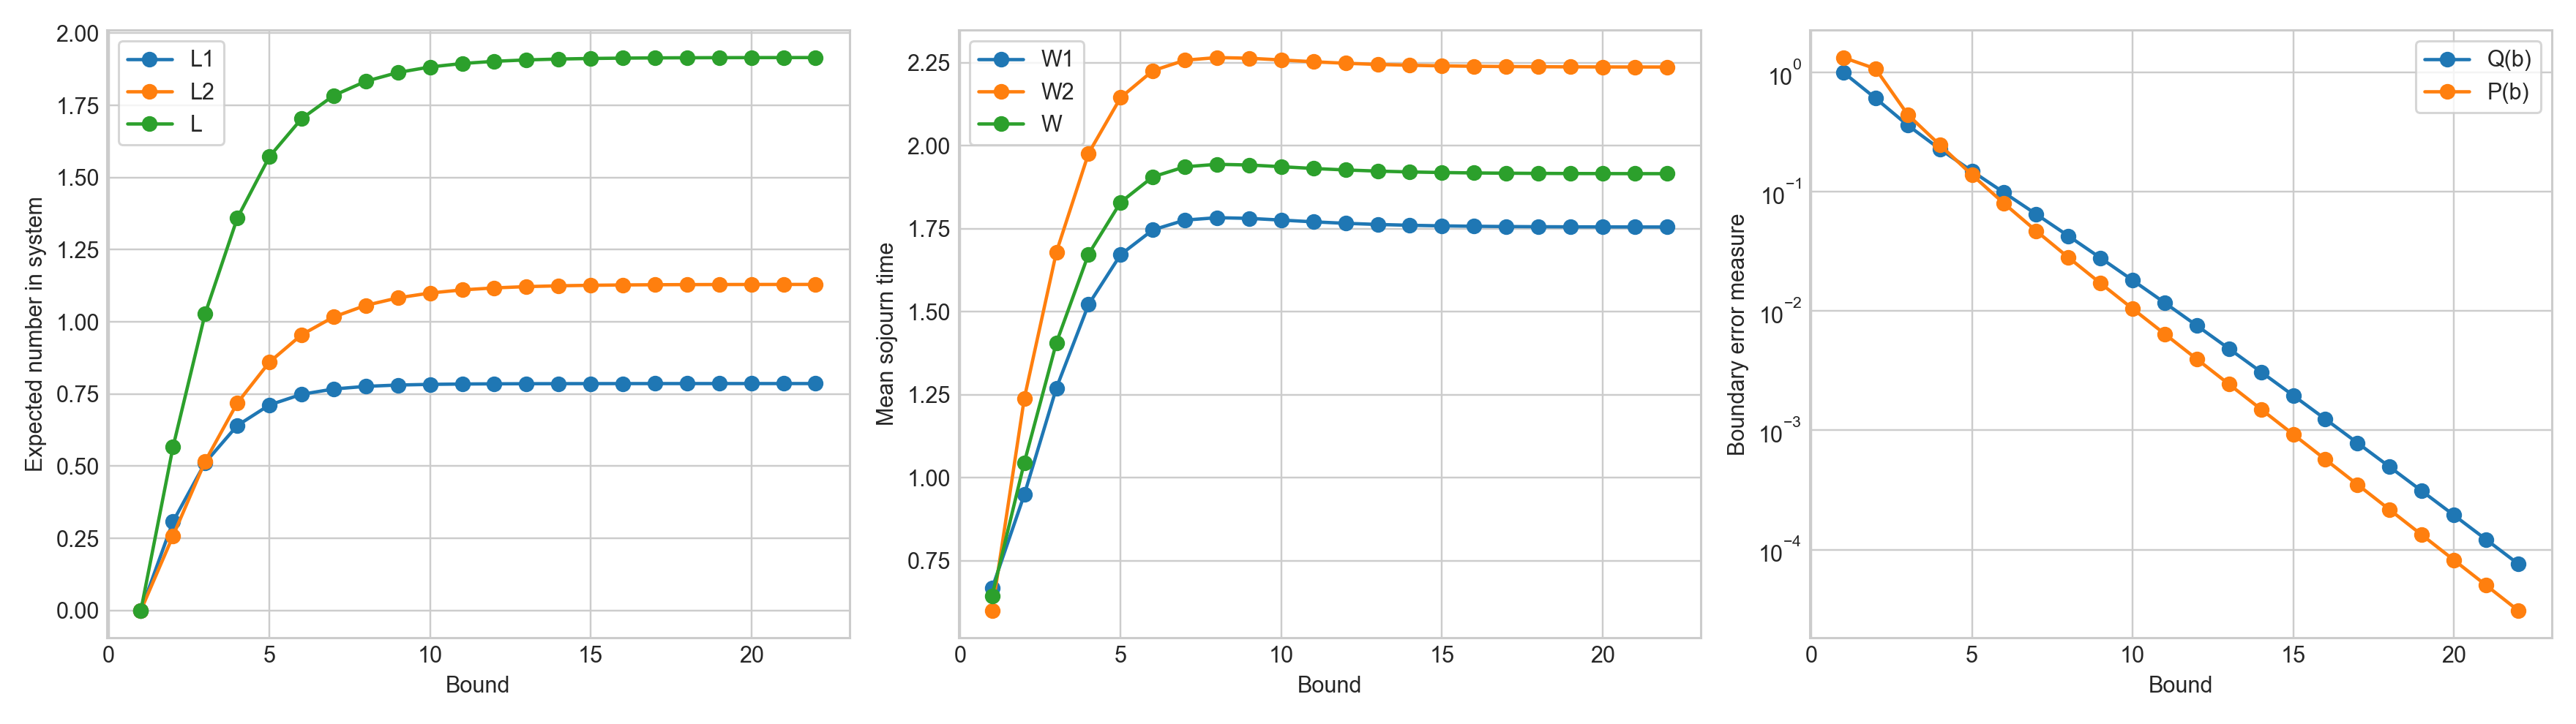
\includegraphics[width=\textwidth]{../results/parameter_variants/original_notebook/bounded_markov_replication.png}
\caption{原始 notebook 参数}
\end{subfigure}
\caption{Bounded Markov approximation 随截断边界的变化。}
\end{figure}

\textbf{判断：\pass。} 这是当前复现中最可靠的一部分。两套参数在较大 bound 下均表现出收敛，边界量下降到 $10^{-4}$ 以下，说明有限截断对稳态均值的影响已经较小。

需要注意的是，低 bound 下 $P(b)$ 在个别点可能超过 1。如果将其字面解释为概率，这是不合理的；更稳妥的表述是：当前代码中的 $P(b)$ 在低边界时可能更像一个边界命中相关的数值诊断量，只有在边界足够大、数值小于 1 时才具有直接概率解释。最终报告中不建议强调低 bound 的 $P(b)$。

\subsection{$H$ 矩阵影响实验}

Effect-of-$H$ 实验在 $h_{12},h_{21}\in[0,3]$、步长 0.2 的 $16\times16$ 网格上计算 $L_k$、$W_k$、variance $U$、$Q(16)$、$P(16)$。三种 service-rate scenario 的边界结果如下：

\begin{table}[H]
\centering
\caption{Effect-of-$H$ 边界量检查}
\begin{tabularx}{\textwidth}{@{}p{0.26\textwidth}ccccX@{}}
\toprule
Scenario & $\max Q(16)$ & $\max P(16)$ & $U_{\min}$ & $U_{\max}$ & 判断 \\
\midrule
A: prioritized class slower & 0.0822 & 0.0120 & 1.704 & 7.927 & $P$ 基本达标，但 $Q$ 明显超过 0.012，181 个网格点超过阈值。\\
B: equal rates & 0.00753 & 0.00114 & 1.022 & 1.966 & $Q$ 与 $P$ 均达标。\\
C: prioritized class faster & 0.0102 & 0.00152 & 0.521 & 2.257 & $Q$ 与 $P$ 均达标。\\
\bottomrule
\end{tabularx}
\end{table}

\textbf{判断：\partialpass。} B、C 两个 scenario 的边界检查支持论文式有限边界设置；A scenario 的 $Q(16)$ 不满足论文中 $Q(16),P(16)<0.012$ 的说法。因此，当前复现可以支持“$H$ 矩阵变化会显著影响 $L$、$W$ 和二阶矩”的定性结论，但不能无保留支持所有 scenario 的边界充分性。

此外，先前生成的 effect-of-$H$ 图标题存在一个小的展示 bug：标题中 scenario 字母来自文件名最后一个字符。代码已经改成取 scenario 名称的第一个字段，例如 A/B/C。这个问题不影响 CSV 数值，但影响图片展示质量。

\subsection{Markov chain vs simulation 验证}

MC-vs-sim 实验用于检查 bounded Markov 结果和离散事件仿真的一致性。当前结果为：

\begin{table}[H]
\centering
\caption{MC-vs-sim 误差范围}
\begin{tabular}{@{}lcc@{}}
\toprule
参数口径 & $W$ 相对误差范围 & 状态分布 Wasserstein 范围 \\
\midrule
论文文本 & 5.93\%--7.68\% & 0.251--0.395 \\
原始 notebook & 4.43\%--6.29\% & 0.104--0.308 \\
\bottomrule
\end{tabular}
\end{table}

\begin{figure}[H]
\centering
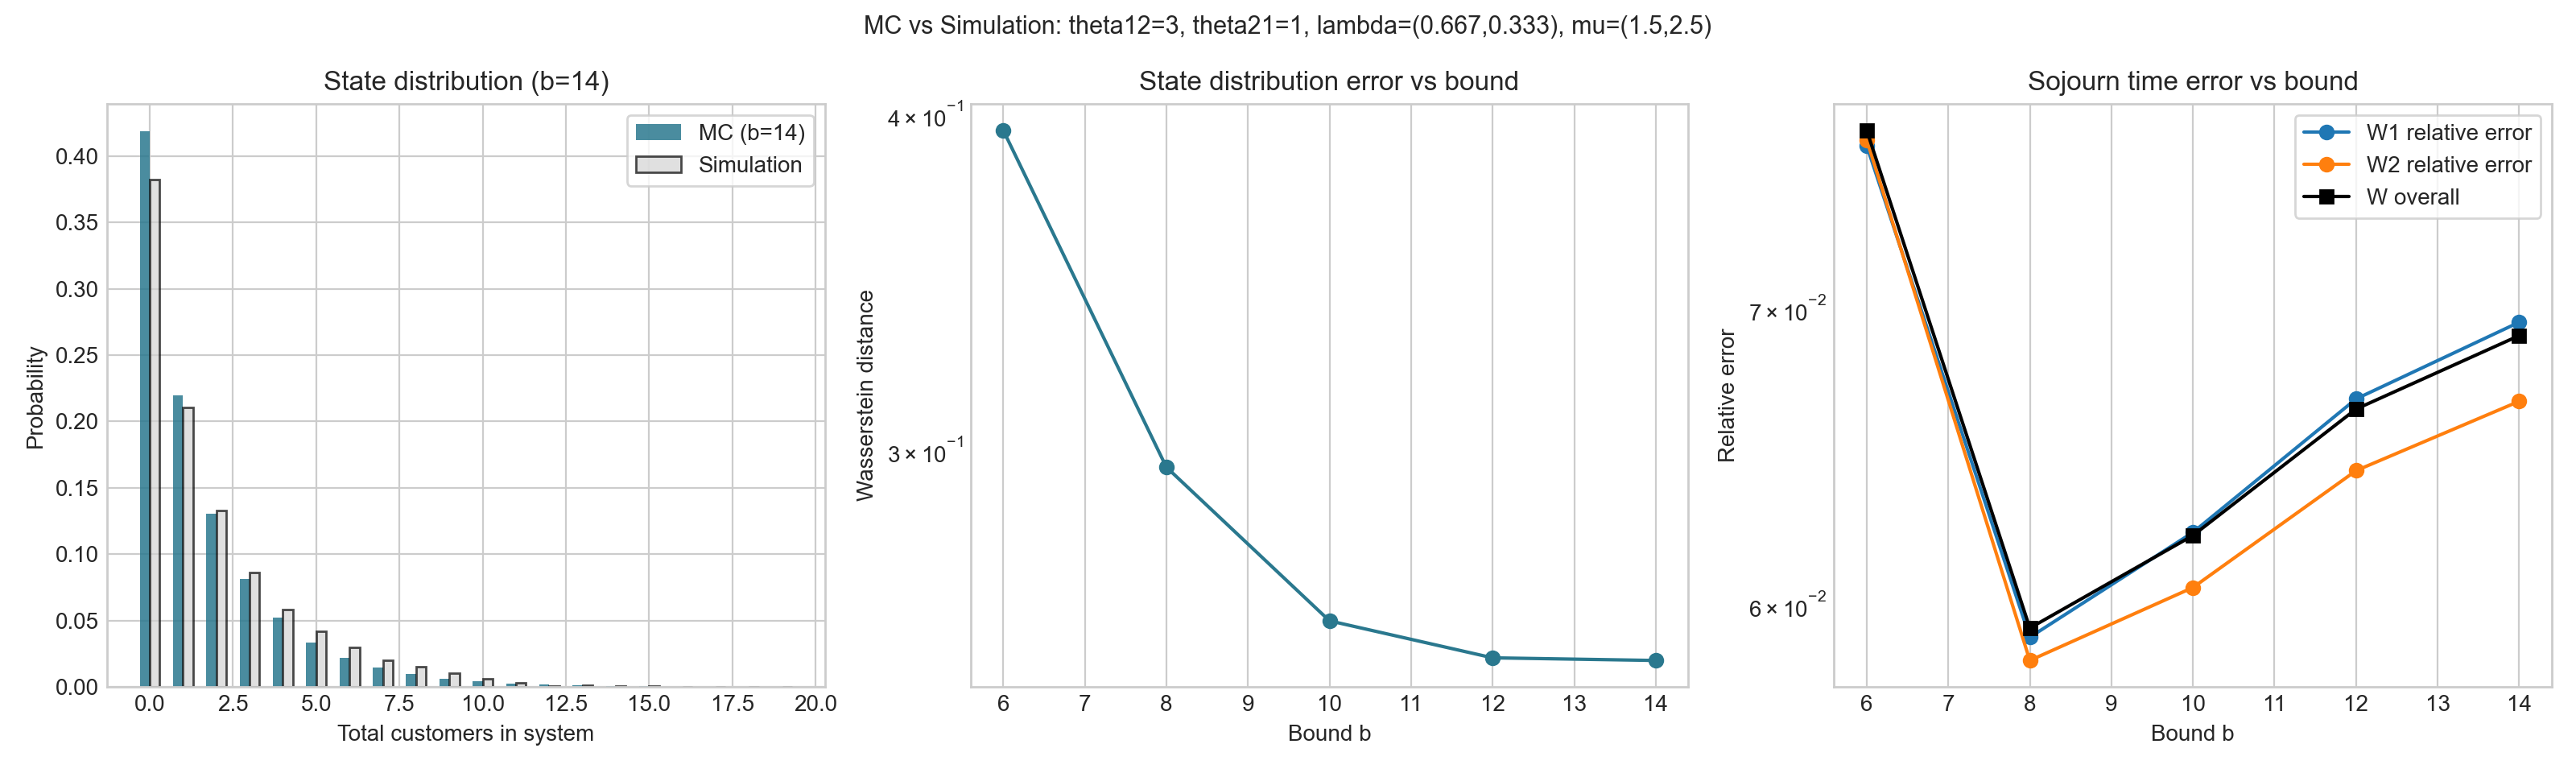
\includegraphics[width=0.82\textwidth]{../results/parameter_variants/paper_text/mc_vs_sim_comparison.png}
\caption{论文文本参数下的 Markov chain vs simulation 比较。}
\end{figure}

\textbf{判断：趋势合理，但证据强度有限。} 状态分布误差整体随 bound 增大而下降，说明 Markov 近似方向正确；但 sojourn-time 均值误差仍在 4\%--8\% 左右，并且并非严格单调。考虑到当前仿真时间为 5000，而论文或原始 notebook 中可能使用更长运行时间，该实验更适合作为 sanity check，不适合作为最终严格验证。

\subsection{Sojourn-time variance 与二阶矩}

Sojourn-time variance 实验基于吸收 Markov 链矩公式计算 $W$ 的方差，并生成 convergence 与 heatmap。当前结果包括：

\begin{table}[H]
\centering
\caption{Sojourn-time variance 关键结果}
\begin{tabular}{@{}lcccc@{}}
\toprule
参数口径 & bound & $W$ & Var$(W)$ & $L$ \\
\midrule
论文文本 & 16 & 1.6216 & 5.6492 & 1.6182 \\
原始 notebook & 16 & 1.9184 & 7.2313 & 1.9138 \\
\bottomrule
\end{tabular}
\end{table}

论文文本参数的 heatmap 中，Var$(W)$ 最小点为 $(h_{12},h_{21})=(3,0)$，Var$(W)=2.0742$；最大点为 $(3,3)$，Var$(W)=6.1467$。原始 notebook 参数下，最小点为 $(0,3)$，Var$(W)=3.9006$；最大点为 $(0.6,0.2)$，Var$(W)=7.4228$。

\begin{figure}[H]
\centering
\begin{subfigure}{0.48\textwidth}
\centering
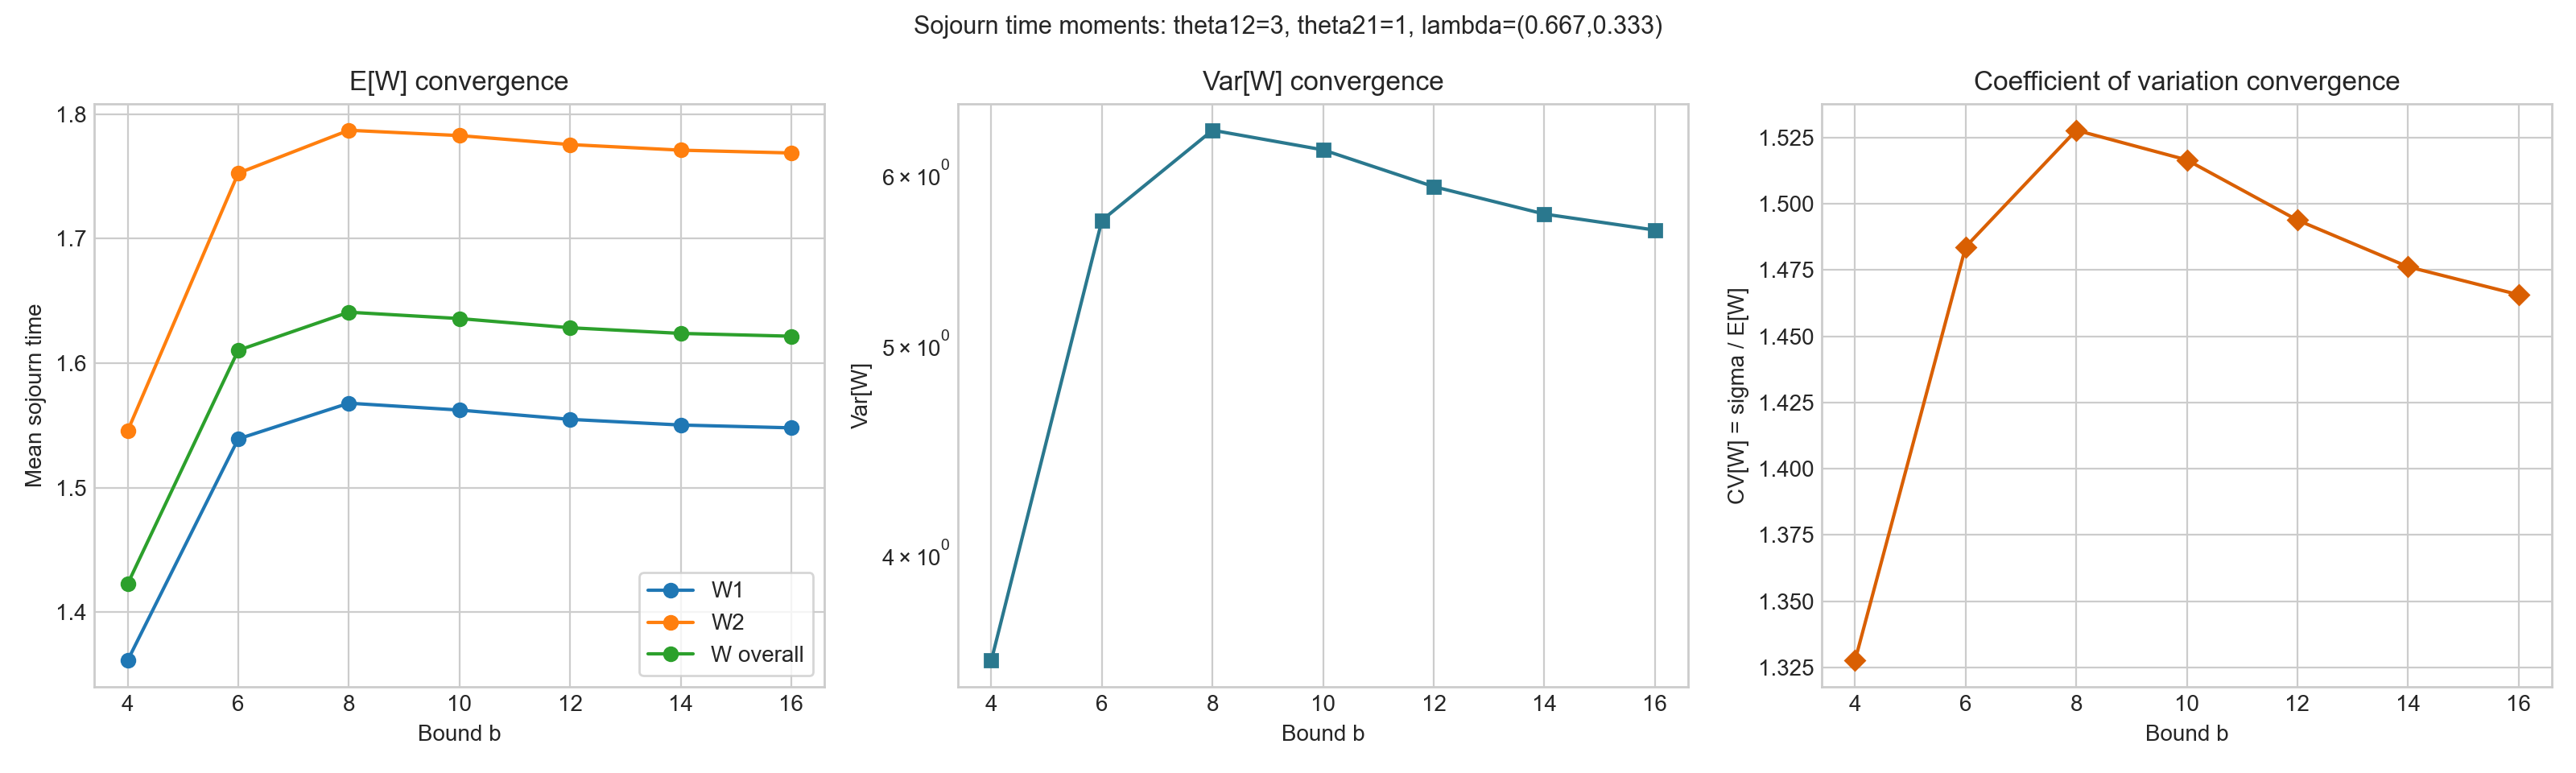
\includegraphics[width=\textwidth]{../results/parameter_variants/paper_text/sojourn_variance_convergence.png}
\caption{Variance convergence}
\end{subfigure}
\hfill
\begin{subfigure}{0.48\textwidth}
\centering
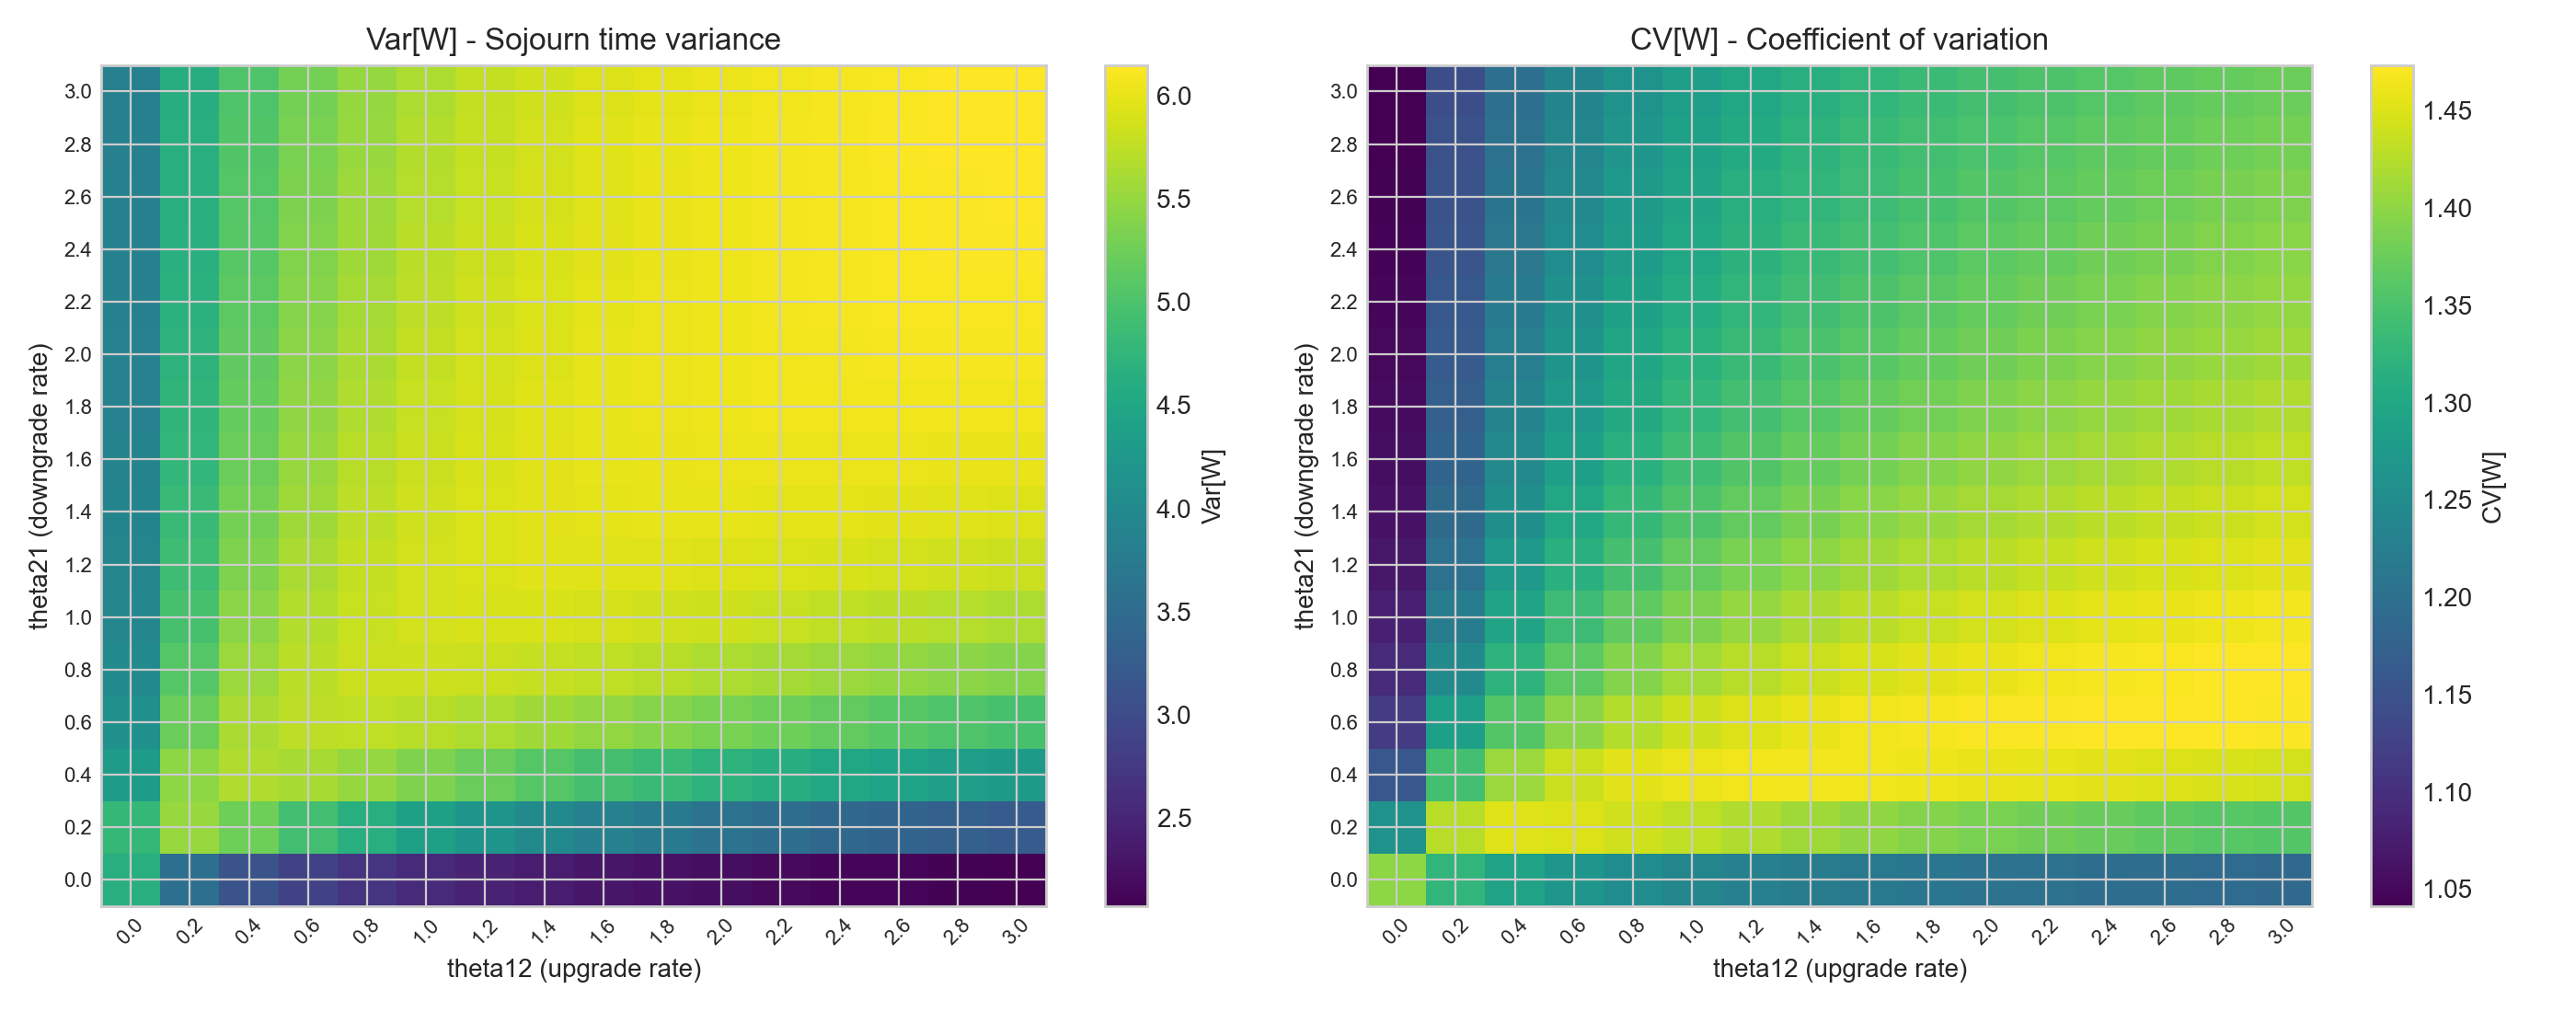
\includegraphics[width=\textwidth]{../results/parameter_variants/paper_text/sojourn_variance_heatmap.png}
\caption{Variance heatmap}
\end{subfigure}
\caption{论文文本参数下的 sojourn-time variance 结果。}
\end{figure}

\textbf{判断：\pass。} 该部分与原论文的吸收链矩公式一致，数值结果也与 bounded Markov 的 $W$、$L$ 结果相互吻合。需要注意的是，sojourn-time variance 本身并不是完全脱离论文的新指标；论文已有二阶矩公式。当前扩展主要体现在更系统地做 convergence/heatmap 可视化。

\section{扩展实验：综合校准指标是否合理}

扩展脚本 \path{reproduction/extension_calibrate_H.py} 使用更细的 $11\times7$ 网格探索 $\theta_{12},\theta_{21}$，并定义
\[
  \text{calibration\_loss}
  =
  \alpha \cdot \text{Wasserstein}
  +
  \beta \cdot \text{MAPE},
  \qquad \alpha=\beta=1.
\]

当前结果如下：

\begin{table}[H]
\centering
\caption{扩展校准实验关键点}
\begin{tabular}{@{}lccc@{}}
\toprule
判据 & 点 $(h_{12},h_{21})$ & Wasserstein & MAPE \\
\midrule
最小综合 loss & $(3,2)$ & 2.6568 & 0.1792 \\
最小 Wasserstein & $(1,2)$ & 2.5763 & 0.2851 \\
最小 MAPE & $(3.5,2)$ & 3.3684 & 0.1084 \\
论文点 & $(3,1)$ & 3.9768 & 0.5179 \\
\bottomrule
\end{tabular}
\end{table}

\begin{figure}[H]
\centering
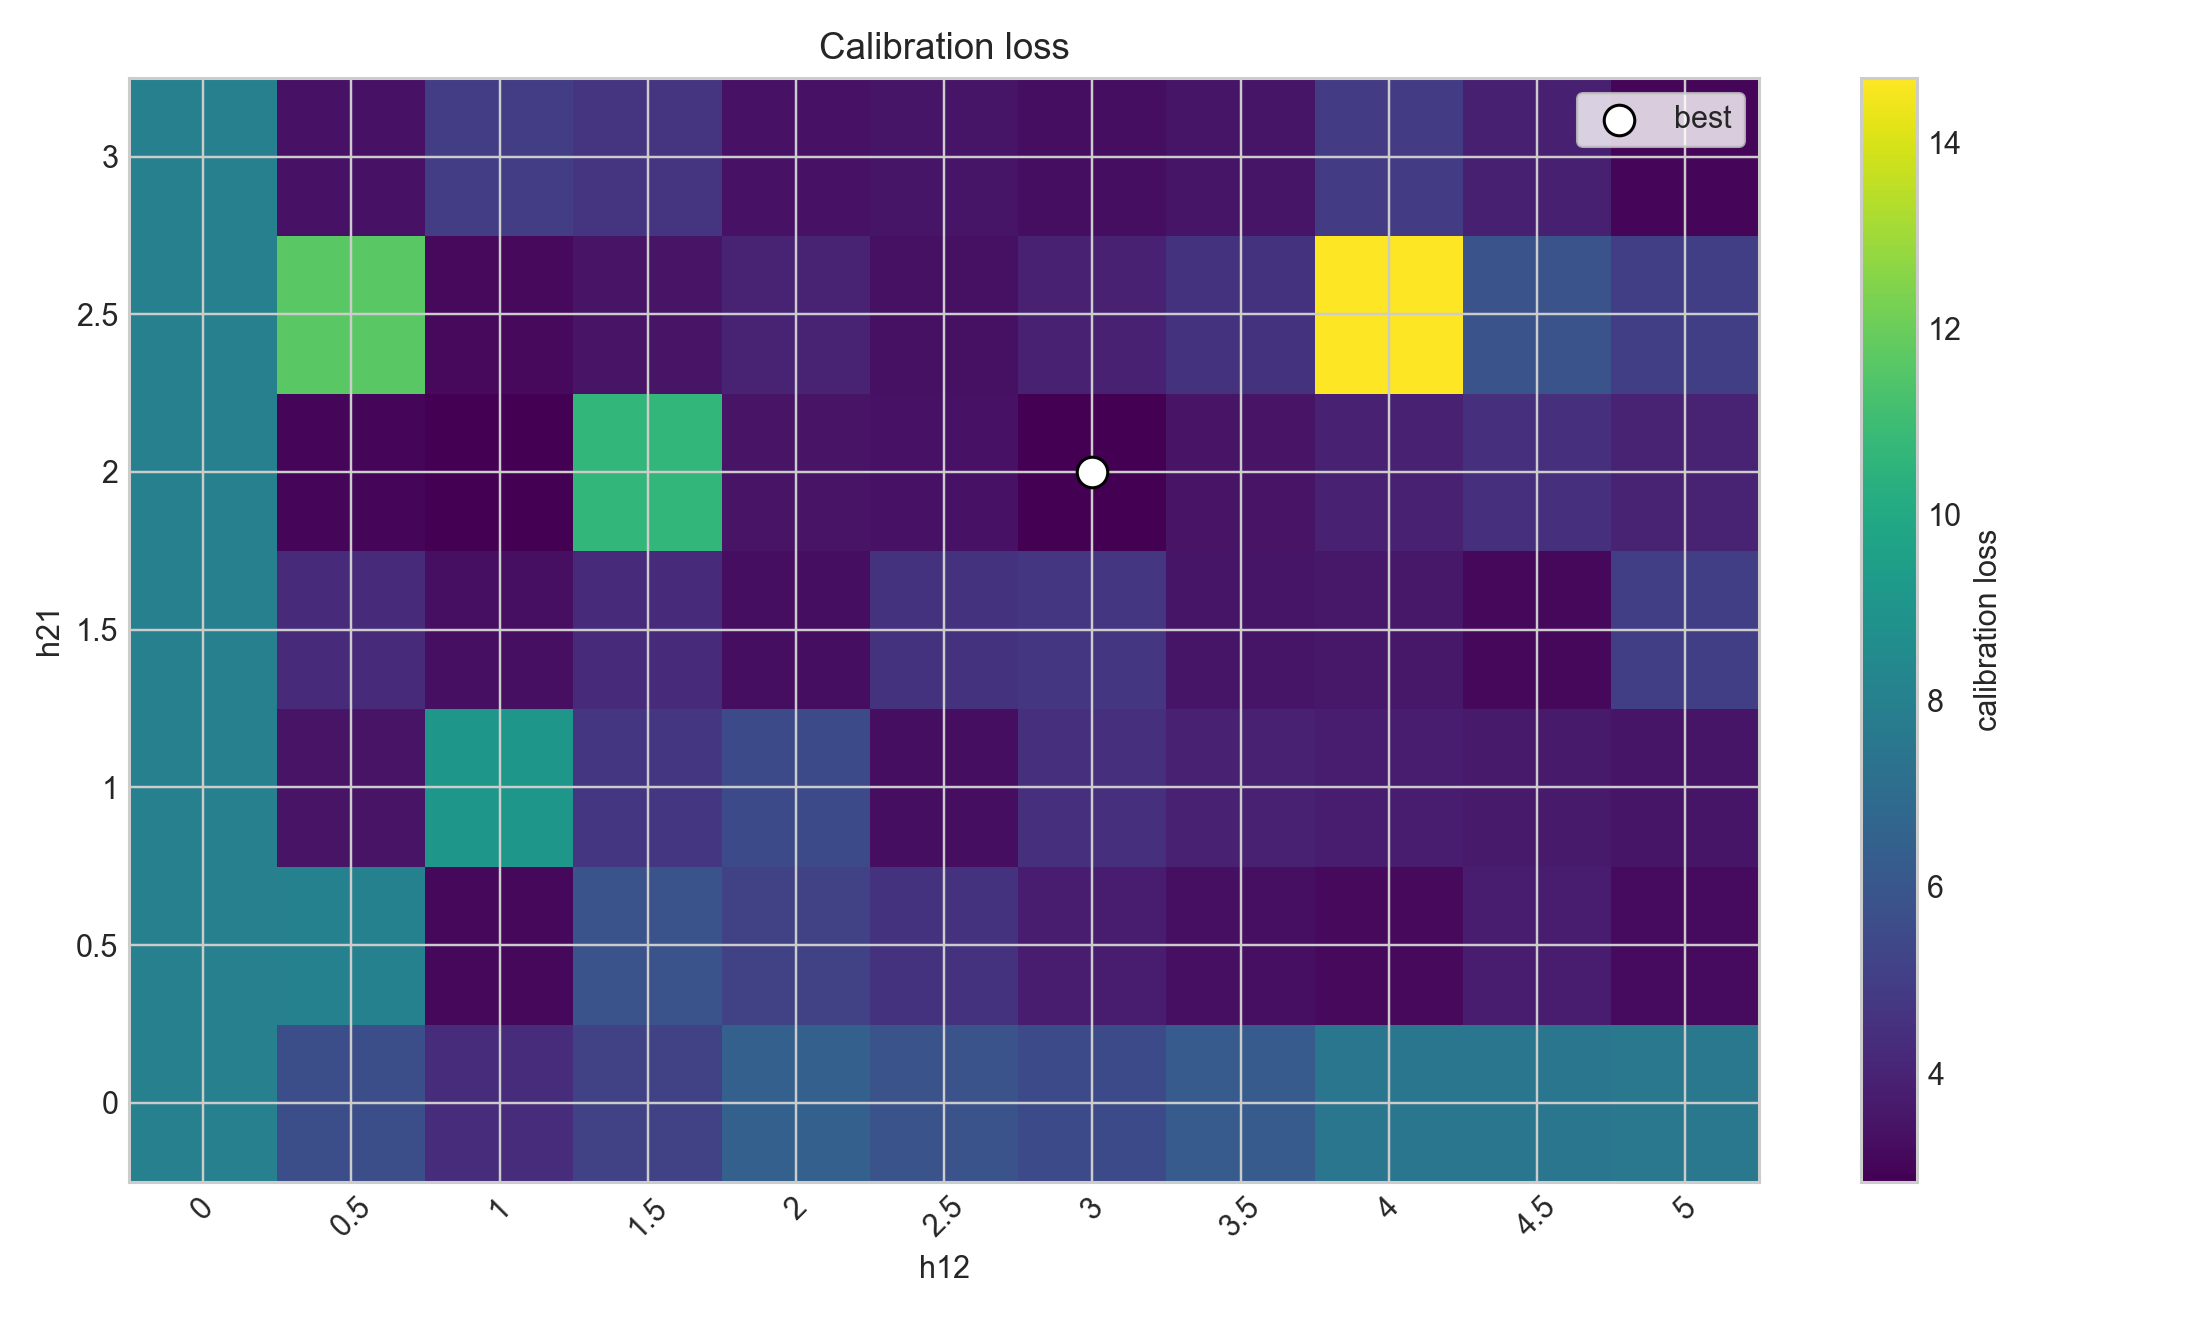
\includegraphics[width=0.65\textwidth]{../results/extension_calibration/extension_calibration_heatmap.png}
\caption{扩展校准综合损失热图。}
\end{figure}

\subsection{这个综合指标有什么用}

综合指标的用途是\textbf{扩展校准}，即在更细的参数网格中快速筛选同时兼顾 distribution shape 和 waiting-time scale 的候选点。Wasserstein distance 主要看 overtaking 分布形状，MAPE 主要看 bumped-up / bumped-down 两类等待时间均值是否接近。把二者线性相加，可以给出一个简单的排序，从而发现“单看一个指标好、另一个指标很差”的点。

\subsection{为什么不应替代论文原始做法}

综合指标不应替代论文复现指标，原因有三点：

\begin{enumerate}
  \item \textbf{不是论文定义的指标。} 论文 Figure 5 对比的是分布形状和等待时间表现，未定义该线性组合 loss。
  \item \textbf{量纲和尺度未归一化。} Wasserstein 和 MAPE 的数值尺度不同，$\alpha=\beta=1$ 是人为选择；当前排序可能由 Wasserstein 主导。
  \item \textbf{trial 数较少。} 当前扩展只用 3 个 trials，适合发现趋势，但不足以作为最终最优参数结论。
\end{enumerate}

因此，最合理的写法是：\textbf{复现部分仍按论文原始指标分别报告；扩展部分另做综合 loss，作为 sensitivity analysis 和参数筛选工具。} 这样既保留复现口径的严谨性，也能说明新增指标的研究价值。

\section{主要问题与修正建议}

\subsection{已经完成或已经纳入当前报告的修正}

\begin{itemize}
  \item 零切换率语义已修正：Ciw 仿真中禁用切换使用 \code{None}，Markov 链计算中使用数值 \code{0.0}。
  \item Figure 5 复现不再使用综合 loss 排序，而是分别报告 Wasserstein 与 MAPE。
  \item 参数变体脚本已支持论文文本和原始 notebook 两套口径。
  \item Bounded Markov 默认 bound 和 service-rate 参数已显式化，便于区分参数来源。
  \item Effect-of-$H$ 绘图标题已修正为 A/B/C scenario 标识。
\end{itemize}

\subsection{仍需谨慎处理的问题}

\begin{itemize}
  \item Figure 5 的 $(3,1)$ 结论未完全复现，建议增加 trials、种子重复和置信区间。
  \item 论文文本稳定性 ADF 检验未通过，建议增加仿真时长、重复轨迹，并比较不同 ADF lag 设定。
  \item Scenario A 的 $Q(16)$ 超阈值，不能直接声称该 bound 对所有 $H$ 网格充分。
  \item MC-vs-sim 的仿真时间较短，当前只能作为 sanity check。
  \item 低 bound 下的 $P(b)>1$ 需要进一步核对原始函数含义，避免误称为概率。
\end{itemize}

\section{最终结论}

从当前结果看，复现工作已经达到“可提交并可解释”的程度，但结论必须诚实分层：

\begin{itemize}
  \item \textbf{强复现：} Bounded Markov approximation；原始 notebook 参数下的 stability split；sojourn-time 二阶矩计算。
  \item \textbf{部分复现：} Figure 5 overtaking fitting；论文文本参数下 stability；effect-of-$H$ 的三种 scenario 中 A 的边界充分性。
  \item \textbf{合理扩展：} fine-grid calibration 和综合 loss；MC-vs-sim validation；variance heatmap。它们 make sense，但需要清楚标注为扩展或诊断，不应作为论文原结论的直接替代。
\end{itemize}

建议最终汇报采用如下表述：本项目成功搭建了完整复现实验框架，并复现了论文中 Markov 链近似和部分稳定性/切换率影响结论；同时，复现实验揭示出论文文本、原始 notebook 与有限仿真设置之间存在若干敏感差异，尤其是 Figure 5 参数排序、稳定性 ADF 检验和 Scenario A 边界量。因此，本复现的贡献不仅是生成图表，也包括识别并解释这些不一致点。

\appendix
\section{本轮实验命令与输出}

本轮完整结果对应的核心命令为：

\begin{verbatim}
python -m reproduction.run_parameter_variants --variant both --include-common
python -m reproduction.extension_calibrate_H
\end{verbatim}

主要输出文件包括：

\begin{itemize}
  \item \path{../results/parameter_variants/common/figure5_metrics.csv}
  \item \path{../results/parameter_variants/common/effect_of_H_A_prioritized_slower.csv}
  \item \path{../results/parameter_variants/common/effect_of_H_B_equal.csv}
  \item \path{../results/parameter_variants/common/effect_of_H_C_prioritized_faster.csv}
  \item \path{../results/parameter_variants/paper_text/stability_metrics.csv}
  \item \path{../results/parameter_variants/original_notebook/stability_metrics.csv}
  \item \path{../results/parameter_variants/paper_text/bounded_markov_metrics.csv}
  \item \path{../results/parameter_variants/original_notebook/bounded_markov_metrics.csv}
  \item \path{../results/extension_calibration/extension_calibration_metrics.csv}
\end{itemize}

\end{document}
